\documentclass[10pt,journal,compsoc]{IEEEtran}
\usepackage[spanish]{babel}
\usepackage[linguistics]{forest}
\usepackage{graphicx}
\usepackage{wrapfig}
\usepackage{listings}
\usepackage{caption}
\ifCLASSOPTIONcompsoc
  \usepackage[nocompress]{cite}
\else
  \usepackage{cite}
\fi

\ifCLASSINFOpdf
\else
\fi
\newcommand\MYhyperrefoptions{bookmarks=true,bookmarksnumbered=true,
pdfpagemode={UseOutlines},plainpages=false,pdfpagelabels=true,
colorlinks=true,linkcolor={black},citecolor={black},urlcolor={black},
pdftitle={Standard ML},
pdfsubject={Tarea Corta 7, Standard ML},
pdfauthor={Daniel, Wilbert, Anthony, Bryan},
}
\renewcommand{\lstlistingname}{Cuadro}
\lstset{
	extendedchars=true,
	frame = single, 
	language=Pascal, 
	framexleftmargin=3pt
}
\hyphenation{op-tical net-works semi-conduc-tor}

\begin{document}
\title{Standard ML}
\author{Daniel~Delgado,~\IEEEmembership{Estudiante,~ITCR,}
        Wilbert~Gonzales,~\IEEEmembership{Estudiante,~ITCR,}
        Anthony~Leandro,~\IEEEmembership{Estudiante,~ITCR,}
        and~Bryan~Mena,~\IEEEmembership{Estudiante,~ITCR}
}
\markboth{Lenguajes de Programaci\'on, Tarea Corta 7 - 24 de octubre, 2017}
{Shell \MakeLowercase{\textit{et al.}}: \LaTex}
\maketitle
\IEEEdisplaynontitleabstractindextext
\IEEEpeerreviewmaketitle
\begin{abstract}
	El presente documento introduce el Standard Meta Language. En la primera secci\'on se explica como inici\'o el lenguaje. En la segunda secci\'on se definir\'an varios tipos de datos b\'asicos.
	
	Es importante aclarar que el prop\'osito de este trabajo no es ser un manual del lenguaje, para esto puede consultarse la bibliograf\'ia m\'as detalladamente.
\end{abstract}

\section{Datos Hist\'oricos}
Standard Meta Language (SML), es un lenguaje de prop\'osito general, modular, funcional con  comprobaci\'on de tipo en tiempo de compilaci\'on e inferencia de tipos. SML es popular entre escritores de compiladores e investigadores de lenguajes de programaci\'on, as\'i como en la demostraci\'on autom\'atica de teoremas.

Las primeras reuniones de dise\'no fueron llevadas a cabo en 1983, 1984 y 1985. A inicios de abril, en Edimburgo, se realiz\'o la reuni\'on inicial con el fin de discutir el primer borrador, realizado por Robin Milner, sobre la propuesta de un lenguaje nuevo, el cual incorporaba ideas de LCF/ML, VAX ML y Hope. Incluyendo a los participantes en f\'isico y de manera virtual, eran 17 los involucrados, algunos de los asistentes fueron Rod Burstall, Luca Cardelli, Kevin Mitchell, entre otros.

\begin{figure}[h]
	\centering
	\captionsetup{justification=centering}
	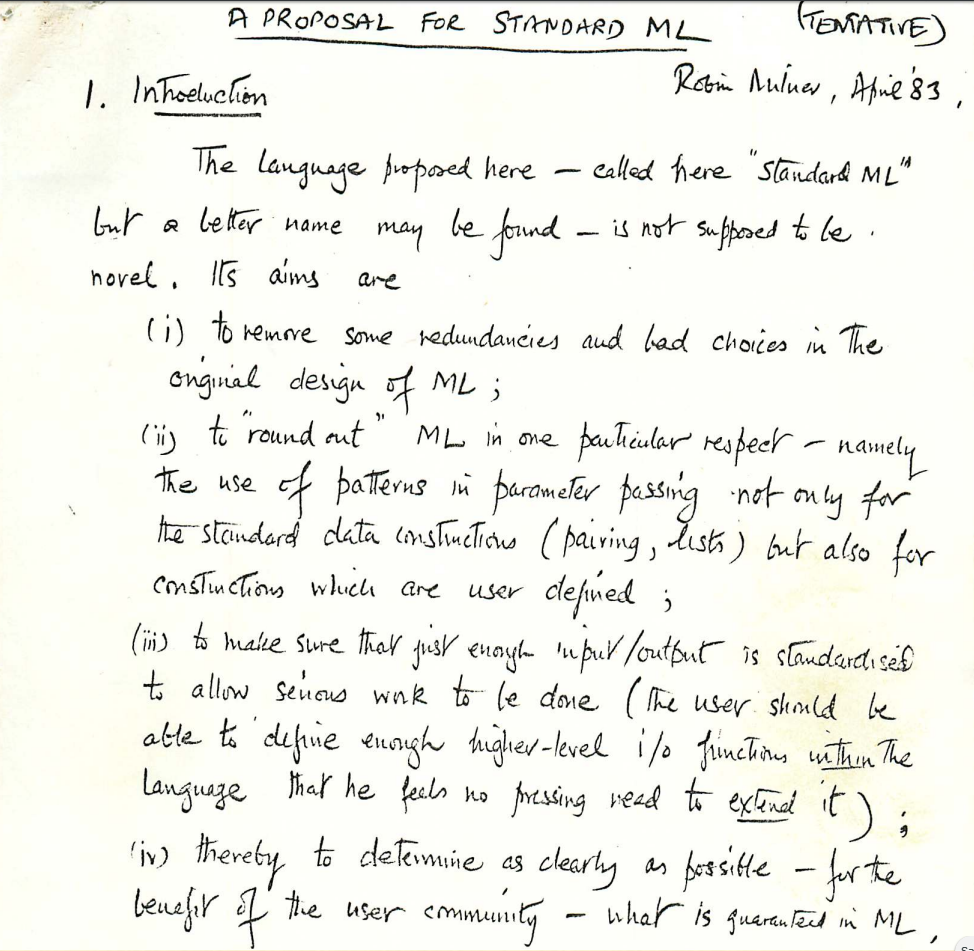
\includegraphics[scale=0.23]{Note.png}
	\caption{Borrador de Robin Milner}
\end{figure}

Desde 1993 hasta el 2000 se efectuaron una serie de reuniones con el objetivo de definir la "siguiente generaci\'on" de ML. Sin embargo no se alcanz\'o un consenso, principalmente por el desacuerdo sobre la idea de agregar o no propiedades de Orientaci\'on a Objetos al lenguaje.

\section{Gu\'ia de Estilo}
\subsection{Identificadores}
\begin{tabular}{c c p{2.5cm}}
	Tipo&Ejemplo&Uso\\
	\hline\hline\\
	Simb\'olico&** ++&Operaciones especiales\\
	Min\'uscula&x y z&Valores locales\\
	Todo en min\'uscula&foo\textunderscore bar&Valores locales\\
	May\'uscula&FooBar&Constructores de tipos, de excepciones, estructuras, functors\\
	Todo en may\'uscula&FOO\textunderscore BAR&Tipo de una estructura\\
	\hline
\end{tabular}

\subsubsection{Convenciones}
\begin{lstlisting}[language=ML, caption=Ejemplo convenciones]
BIEN:
x : 'a 
xs : 'a list 
xss : 'a list list

MAL:
l : 'a list 
list : 'a list
\end{lstlisting}

\subsection{Formato}
\subsubsection{Par\'entesis}
\begin{lstlisting}[language=ML, caption=Convenci\'on par\'entesis]
BIEN:
(x + y)

MAL:
( x + y )
\end{lstlisting}
\subsubsection{Operadores}
\begin{lstlisting}[language=ML, caption=Convenci\'on operadores]
BIEN:
x + y

MAL:
x+y
\end{lstlisting}
\subsubsection{Espacios en blanco}
\begin{lstlisting}[language=ML, caption=Convenci\'on espacios en blanco]
BIEN:
[x, y, z]

MAL:
[x,y,z] 
[x , y , z]
\end{lstlisting}

\subsubsection{Identaci\'on}
Por defecto el tama\'no de la identaci\'on es de dos espacios.
\begin{lstlisting}[language=ML, caption=Convenci\'on identaci\'on]
BIEN:
if b then e1 else e2

if b1 then e1
else if b2 then e2
else e3

if b1 then
  e1
else if b2 then
  e2
else
  e3

MAL:
if b then e1
  else if b2 then e2
    else e3
\end{lstlisting}

\subsection{Recomendaciones generales}
\begin{itemize}
	\item Usar nombres cortos para valores locales.
	\item Es preferible utilizar nombres largos que nombres poco representativos.
\begin{lstlisting}[language=ML, caption=Recomendaci\'on nombres]
BIEN:
fun remueve_duplicados xs = ...	

MAL:
(*esta funci\'on elimina
duplicados de una lista*)
fun procesa_lista xs = ...
\end{lstlisting}
	\item Evitar comentarios sin sentido.
\begin{lstlisting}[language=ML, caption=Recomendaci\'on comentarios]
MAL:
(*esta funci\'on elimina
duplicados de una lista*)
fun remueve_duplicados xs = ...	
\end{lstlisting}
	\item Nunca mezclar convenciones en definici\'on de nombres.
	\item Nunca mezclar idiomas en el c\'odigo.
\end{itemize}

\section{Tipos de Datos}
Existen diferentes tipos b\'asicos pre-definidos en SML. Por ejemplo el tipo de valores l\'ogicos, llamado \textit{bool}. Esto tiene exactamente dos valores, verdadero o falso. Otro tipo simple es el \textit{string}. Los \textit{strings} se colocan entre comillas dobles (como en ''Hola'') y se unen con '' $\wedge$  '' (el símbolo del cursor o flecha hacia arriba). Como era de esperar, la expresión ''Hola'' $\wedge$ ''mundo!'' se eval\'ua como ''Hola mundo!''. Tambi\'en hay un tipo \textit{char} para caracteres individuales. Una constante \textit{char} es una constante \textit{string} de longitud uno precedida por un s\'imbolo de hash. As\'i, \#''a'' es la letra a. Se puede acceder a los caracteres de ocho bits mediante su c\'odigo ASCII.

Los tipos numéricos en SML son los enteros de tipo \textit{int}, los n\'umeros reales de tipo \textit{real} y enteros sin signo (o palabras) de tipo \textit{word}. Adem\'as de esto, una implementaci\'on del lenguaje puede proporcionar otros tipos num\'ericos en una biblioteca, por ejemplo, enteros de precisi\'on arbitraria, reales de doble precisi\'on o incluso bytes (enteros sin signo de 8 bits). Los n\'umeros enteros se pueden representar en notaci\'on decimal o hexadecimal, de modo que 255 y 0xff representan el n\'umero entero 255.

Los tipos num\'ericos mencionados son tipos separados y deben usarse funciones para convertir un entero a un real o un word a un byte. No hay conversi\'on impl\'icita entre tipos como en otros lenguajes de programaci\'on.

\subsection{Estructuras B\'asicas de datos}
\begin{itemize}
	\item Num\'ericos
		\subitem \textbf{int} (integer), como un $\sim$7 o 255. N\'otese que una virgulilla '$\sim$' es usada para n\'umeros negativos.
		\subitem \textbf{real} (n\'umero de punto flotante), como un $\sim$7.8 o 9.4. 
		
		\subitem SML no hace conversiones num\'ericas entre int y real autom\'aticamente. Por lo tanto una expresi\'on como 9 + 3.66 es inv\'alida. Debe ser escrito como 9.0 + 3.66, o real(9) + 3.66 (usando la funci\'on real para convertir 9 a 9.0).
		
	\item Caracteres
		\subitem \textbf{string} (cadena de caracteres), como ''esto es una cadena'' o ''''. N\'otese que el segundo es una cadena vac\'ia, contiene cero caracteres.
		\subitem \textbf{char} (un caracter), como \#''y''.
	
	\item L\'ogico
		\subitem \textbf{bool} (valor Booleano), este puede ser verdadero o falso.
\end{itemize}		
\subsection{SML Basis Library}
La biblioteca \textit{SML Basis} es el est\'andar para la revisi\'on de SML en 1997. Esta biblioteca provee interfaces y operaciones para tipos b\'asicos, como integers y strings, soporte para entrada y salida, soporte para tipos de datos est\'andar, como lo son \textit{options} y las listas. Algunas de las funciones de esta biblioteca son:
\begin{itemize}
	\item Constantes matem\'aticas b\'asicas como ra\'iz cuadrada, funciones trigonom\'etricas, hiperb\'olicas, exponenciales y logar\'itmicas.
	\item Tener en un \textit{real} valores positivos o negativos infinitos.
	\item Conversi\'on de valores booleanos a \textit{string}.
	\item Representaci\'on e intervalos de tiempo.
	\item Conversiones entre valores num\'ericos.
	\item B\'usquedas en cadenas de \textit{char}.
	\item Operaciones sobre \textit{strings}.
	\item Operaciones sobre listas.
	\item Obtener valor absoluto.
	\item Longitud de un array.
\end{itemize}

\subsection{Opciones}
El tipo de dato \textit{option} puede utilizarse cuando es posible que algo no tenga un valor v\'alido. Por ejemplo, una divisi\'on entre cero, sin tener que recurrir al manejo de excepciones.
\begin{lstlisting}[language=ML, caption=Ejemplo Divisi\'on entre 0]
fun dividir x y = if y == 0
then NONE else SOME (x / y)
\end{lstlisting}

\subsection{Listas}
Las listas en SML son un tipo de dato recursivo y polim\'orfico; sumamente importantes y comunes en la programaci\'on funcional. La estructura de una lista es la siguiente: cabeza (head) se encuentra en la primer posici\'on (de izquierda a derecha) y la cola (tail) corresponde al resto de elementos. Cada elemento de la lista tiene un \'indice, iniciando con el valor 0 para la cabeza.
\begin{lstlisting}[language=ML, caption=Ejemplo Listas]
datatype 'a list = nil
| :: of 'a * 'a list
\end{lstlisting}
'::' es un operador infijo, por ejemplo, \textit{3 :: 4 :: 5 :: nil} es una lista de tres enteros (int). Tambi\'en es posible declarar listas de la siguiente forma: \textit{[3, 4, 5]}.

\subsection{Tuplas}
Los tipos de datos, incluidos los tipos b\'asicos anteriores, se pueden combinar de diferentes maneras. Una forma de hacer esto es en una tupla, que es un conjunto ordenado de valores; por ejemplo, la expresi\'on (1, 2) es del tipo int * int, y ('foo', false) es del tipo string * bool. Tambi\'en hay una 0-tupla, (), cuyo tipo se denomina \textit{unit}.
Las tuplas pueden ser anidadas, y (a diferencia de algunos formalismos matem\'aticos), (1, 2, 3) es distinto de ((1, 2), 3) y de (1, (2, 3)). El primero es de tipo int * int * int; los otros dos son de tipos (int * int) * int e int * (int * int), respectivamente. Ejemplos de declaraciones de tuplas:
\begin{lstlisting}[language=ML, caption=Ejemplo Listas]
val alien1 = ("Groot", 1586, 3.14159)

val gustos = 
[ ("Gamora", "helados"),
("Drax",   "perritos"),
("Rocket",   "cerrezas") ]

val combinado = 
[ ("Gamora", 27),
("Drax",   78),
("Rocket",   15) ]

val articulos =
(["helado", "perritos",
 "chocolate"], ["higado", 
 "alquiler" ])
\end{lstlisting}

\subsection{Tokens}
Un programa escrito en SML consiste de una secuencia de \textit{tokens}, algunos de los m\'as comunes son:
\begin{tabular}{c p{3cm} p{5cm}}
	Tipo de token & Ejemplos\\
	\hline\hline\\
	Identificadores alfanum\'ericos & x, mod, 'a\\
	Identificadores simb\'olicos & +, -, *, /\\
	Constantes especiales & 2, ~5.6, "string", \#'c'\\
	Palabras clave & val, =, (, )\\
	\hline
\end{tabular}

\section{Funciones}
En SML una funci\'on acepta un valor y normalmente devuelve otro valor. Como puede verse en el cuadro 11 la funci\'on factorial es de tipo \textit{int $\rightarrow$ int}, esto significa que la funci\'on recibe un valor de tipo \textbf{int} y retorna un valor de tipo \textbf{int}. El \textit{binding} para la funci\'on debe hacerse como el ejemplo.

\begin{lstlisting}[language=ML, caption=Ejemplo Factorial]
fun factorial n =  if n < 1  
then 1  else n * factorial (n - 1)
\end{lstlisting}

Incluso si una funci\'on no retorna un valor en tiempo de ejecuci\'on (por una excepci\'on o si entra a un loop infinito) tiene un tipo de retorno est\'atico en tiempo de compilaci\'on. Es importante recordar que las funciones en SML son valores y todos los valores pueden estar enlazados a nombres, por lo tanto funciones pueden estar enlazadas a nombres.

Cuando en el cuerpo de una funci\'on no se provee de suficiente informaci\'on para determinar el tipo exacto del argumento de retorno, puede definirse el tipo expl\'icitamente de la siguiente manera:

\begin{lstlisting}[language=ML, caption=Ejemplo Factorial Tipo Expl\'icito]
fun factorial (n : int) : int = if n<1
then 1  else n * factorial (n - 1)
\end{lstlisting}

\subsection{Comprobaci\'on de tipos}
Los tipos de las llamadas a funciones son comprobadas de la manera m\'as obvia. El argumento actual debe coincidir con el argumento formal, cuando no es as\'i se genera un error.

\subsection{Funciones sin valores de retorno o argumentos}
Lenguajes como Pascal resuelven este problema dividiendo el universo de abstracciones de control en dos tipos: funciones, que devuelven valores y procedimientos, que no. Los lenguajes como C solucionan este problema al tener funciones \textit{void} que no devuelven nada. SML utiliza un enfoque similar, pero no igual a este \'ultimo: utiliza el tipo \textit{unit}, que tiene un valor, escrito (): \textit{printHi()}

\subsection{Funciones recursivas}
Las funciones recursivas son aquellas que utilizan alg\'un tipo de iteraci\'on para obtener los resultados. En los lenguajes imperativos la iteraci\'on se logra utilizando ciclos \textit{while} y ciclos \textit{for}, en SML se hace mediante la recursi\'on.

Una funci\'on definida por recursi\'on es una que calcula el resultado de una llamada "llam\'andose a s\'i misma". Para hacer esto la funci\'on debe tener un nombre con el cual se har\'a referencia a la misma. Se logra usando un \textit{binding} de valor recursivo.

\textit{Bindings} de valor recursivo tienen casi la misma forma que los ordinarios, excepto que el \textit{binding} es calificado con el adjetivo "rec", como en el ejemplo siguiente:

\begin{lstlisting}[language=ML, caption=Ejemplo Factorial Recursivo]
val rec factorial : int->int = fn 0=>1
| n:int => n * factorial (n-1)
\end{lstlisting}

Usando la notaci\'on de \textit{fun} puede escribirse m\'as claramente y conciso as\'i:

\begin{lstlisting}[language=ML, caption=Ejemplo Factorial Recursivo Fun]
fun factorial 0 = 1
|factorial (n:int) = n*factorial (n-1)
\end{lstlisting}

En ciertas ocasiones es \'util definir dos funciones simult\'aneamente, donde cada una se llama a s\'i misma o a la otra funci\'on para calcular el resultado. Este tipo de funciones se les llama \textit{mutuamente recursivas}, esto se hace de la siguiente manera:

\begin{lstlisting}[language=ML, caption=Ejemplo Funciones Mutuamente Recursivas]
fun par 0 = true
| par n = impar (n-1)
and impar 0 = false
| impar n = par (n-1)
\end{lstlisting}

\subsection{Ramificaci\'on (branching)}
Los lenguajes imperativos expresan ramificaci\'on a trav\'es de declaraciones condicionales, sin embargo lenguajes funcionales como SML, expresan ramificaci\'on principalmente a trav\'es de expresiones condicionales.

\subsection{Expresiones if}
Los condicionales if en SML tienen la siguiente sintaxis: \textit{if boolExpr then expr1 else expr2}

Esto tiene la sem\'antica similar al operador :? de C:
\begin{enumerate}
	\item Primero, boolExpr es evaluado.
	\item Si la expresi\'on es verdadera, entonces expr1 es evaluada y retornada.
	\item Si la expresi\'on es falsa, entonces la expr2 es evaluada y retornada.
\end{enumerate}

\subsection{Secuenciadores (sequencing)}
Las secuencias de expresiones en SML son escritas separadas por punto y coma entre par\'entesis.

Secuencias de expresi\'on tienen la siguiente sem\'antica:

\begin{enumerate}
	\item Evaluar cada expresi\'on en orden de izquierda a derecha.
	\item Devuelven la \'ultima expresi\'on evaluada como el valor de toda la expresi\'on.
\end{enumerate}

Todos los resultados aparte de la \'ultima expresi\'on son descartados. Las secuencias de expresiones son primordialmente \'utiles para las expresiones de efectos secundarios como \textit{print}:


\begin{lstlisting}[language=ML, caption=Ejemplo Secuencias de Expresiones]
- val x = (print "Hola\n"; 7)

Output:
Hola
val x = 7 : int
\end{lstlisting}

\subsection{Comparaci\'on de patrones}
La expresi\'on if b\'asicamente provee una manera de igualar un valor booleano contra un verdadero o falso. Otra manera de escribir esto en SML es:

\begin{lstlisting}[language=ML, caption=Ejemplo Secuencias de Expresiones]
case boolExpr of
true => expr1
| false => expr2
\end{lstlisting}

El constructo case toma un valor e intenta igualarlo a uno o m\'as patrones, en este caso, los dos patrones constantes booleanos, falso y verdadero. Si un patr\'on es igual, entonces su correspondiente funci\'on es evaluada y retornada como el valor de la expresi\'on completa. Los patrones son probados de izquierda a derecha.

Los patrones no est\'an restringidos a ser usados en declaraciones \textit{case}. Podr\'ian aparecer donde cualquier \textit{binding} aparezca, incluyendo declaraciones \textit{val} y argumentos de funciones.

\subsection{Polimorfismo}
En muchos lenguajes de programación (por ejemplo, Java) encontramos que terminamos reescribiendo el mismo c\'odigo una y otra vez para que funcione con diferentes tipos. SML no tiene este problema, pero tenemos que introducir nuevas caracter\'isticas para mostrar c\'omo evitarlo. Supongamos que queremos escribir una funci\'on que intercambia la posici\'on de valores en un par ordenado:

\begin{lstlisting}[language=ML, caption=Ejemplo Polimorfismo 1]
fun swapInt(x: int, y: int):
int*int = (y,x)

fun swapReal(x: real, y: real):
real*real = (y,x)

fun swapString(x: string, y: string):
string*string = (y,x)
\end{lstlisting}

Esto es tedioso, porque estamos escribiendo exactamente el mismo c\'odigo cada vez. ?`Qu\'e sucede si los elementos de dos pares tienen diferentes tipos?

\begin{lstlisting}[language=ML, caption=Ejemplo Polimorfismo 2]
fun swapIntReal(x: int, y: real):
real*int = (y,x)

fun swapRealInt(x: real, y: int):
int*real = (y,x)
\end{lstlisting}

La mejor manera de hacer esto es:

\begin{lstlisting}[language=ML, caption=Ejemplo Polimorfismo correcto]
- fun swap(x: 'a, y: 'b):
 'b * 'a = (y,x)
 
val swap = fn :
 'a * 'b -> 'b * 'a
\end{lstlisting}

En lugar de escribir tipos expl\'icitos para x e y, se escriben las variables de tipo 'a y b'. El tipo de swap es 'a*'b$\rightarrow$'b*'a. Lo que esto significa es que podemos usar \textit{swap} como si tuviera cualquier tipo que se pudiese obtener consistentemente reemplazando 'a' y 'b' en su tipo con un tipo para 'a y un tipo para 'b. Puede usarse el nuevo \textit{swap} en lugar de todas las viejas definiciones:

\begin{lstlisting}[language=ML, caption=Ejemplo Polimorfismo con definiciones antiguas]
(*swap:(int*int)->(int*int)*)
swap(1,2);

(*swap:(real*real)->(real*real)*)
swap(3.14,2.17);

(*swap:(string*string)->(string*string)*)
swap("foo","bar");  

(*swap:(string*real)->(real*string)*)
swap("foo",3.14);   
\end{lstlisting}

Esta capacidad de usar \textit{swap} como si tuviera muchos tipos diferentes se conoce como polimorfismo, del griego para "muchas formas". Si pensamos que \textit{swap} tiene una "forma" que su tipo define, entonces \textit{swap} puede tener muchas formas: es polim\'orfico. Obs\'ervese que el requisito de que las variables de tipo sean sustituidas consistentemente significa que algunos tipos est\'an descartados; por ejemplo, es imposible usar swap en el tipo (int * real) $\rightarrow$ (string * int), porque ese tipo sustituir\'ia consistentemente por la variable de tipo 'a pero no por 'b.

Los programadores de SML suelen leer los tipos 'a' y 'b' como~\textquotedblleft alfa\textquotedblright~y "beta". Esto es m\'as f\'acil que decir~\textquotedblleft comillas simples a". De hecho, una variable de tipo puede ser cualquier identificador precedido por una comilla simple; por ejemplo, el valor \textit{'key} y \textit{'valor} tambi\'en son variables legales. El compilador SML necesita tener estos identificadores precedidos por una comilla simple para que sepa que est\'a viendo una variable de tipo.

Es importante tener en cuenta que el \textit{swap} no utiliza sus argumentos \textit{x} o \textit{y} de manera interesante. Los trata como si fueran cajas negras. Cuando el verificador de tipo SML est\'a comprobando la definici\'on de \textit{swap}, todo lo que sabe es que \textit{x} es de alg\'un tipo arbitrario 'a. No permite realizar ninguna operaci\'on en \textit{x} que no pueda realizarse en un tipo arbitrario. Esto significa que el c\'odigo est\'a garantizado para trabajar para cualquier x e y.

\section{Caracter\'isticas}
\begin{itemize}
\item SML cuenta con un sistema de tipado est\'atico particularmente fuerte. A diferencia de muchos lenguajes, no tiene subtipos (relaciones 'is-a') o impl\'icitos entre tipos.

\item El t\'ermino \textit{strong typing} se utiliza en una amplia variedad de maneras diferentes; no obstante, es justo decir que SML proporciona tipificaci\'on fuerte por casi todas las definiciones. 

\item Cada expresi\'on en un programa SML tiene un tipo espec\'ifico en tiempo de compilaci\'on y su tipo en tiempo de ejecuci\'on nunca se contrapone a esto.

\item Todas las conversiones de tipos son expl\'icitas (utilizando funciones como \textit{real}, que acepta un n\'umero entero y devuelve un n\'umero real equivalente), y toman la forma de traducciones significativas en lugar de meras reinterpretaciones de bits en bruto.

\item La mayor\'ia de los lenguajes no se adhieren estrictamente a uno solo de los enfoques de tipado, sino m\'as bien, utilizan elementos de m\'as de uno. El sistema de tipos de SML, sin embargo, usa la tipificaci\'on est\'atica casi exclusivamente. 

\item Un programa mal tipificado ni siquiera compilar\'a. En la medida en que SML admite el tipo din\'amico, es dentro del marco de tipificaci\'on est\'atica.
\end{itemize}


\section{Ventajas}
\begin{itemize}
	\item Permite a los programadores definir tipos de datos abstractos.
	\item Los programadores de SML consideran el estilo de tipado de SML un aspecto positivo, ya que permite que muchos errores de programaci\'on sean capturados en tiempo de compilaci\'on que un lenguaje de tipo din\'amico solo captura en tiempo de ejecuci\'on.
	\item En SML/NJ se puede construir y manejar estructuras de datos de C arbitrarias en c\'odigo SML.
	\item En SML/NJ Puede cargar bibliotecas de C y encontrar funciones/variables en tiempo de ejecuci\'on.
	\item En SML/NJ Puede administrar memoria de estructuras de datos de C. Si se sabe que algo no se usa, puede liberarse.
\end{itemize}

\section{Desventajas}
\begin{itemize}
	\item Si el programador se encuentra acostumbrado a los dem\'as lenguajes donde el tipado es distinto, encontrarse con SML puede significar un mayor tiempo en el aprendizaje de este.
	\item Los tipos, en comparaci\'on con otros lenguajes, son un poco m\'as complejos de comprender.
\end{itemize}

\section{C\'odigo de ejemplo}
El programa "hello.sml"

\begin{lstlisting}[language=ML, caption=Ejemplo Hello World]
print "Hello, World!\n";
\end{lstlisting}

Puede compilarse con MLton:

\begin{lstlisting}[language=ML, caption=Compilar Hello World]
$ mlton hello.sml
\end{lstlisting}

Y ejecutarse:

\begin{lstlisting}[language=ML, caption=Ejecuci\'on Hello World]
./hello

Hello, World!
\end{lstlisting}

\begin{thebibliography}{1}
	\bibitem{1}
	CSE341 Lecture Notes 3: Functions and patterns in ML. (s. f.). Recuperado 3 de octubre de 2017, a partir de https://courses.cs.washington.edu/courses/cse341/04wi/lectures/03-ml-functions.html
	
	\bibitem{2}
	Learn Standard ML in Y Minutes. (s. f.). Recuperado 18 de septiembre de 2017, a partir de https://learnxinyminutes.com/docs/standard-ml/
	
	\bibitem{3}
	Lecture 4: Polymorphism and Parameterized Types. (s. f.). Recuperado 6 de octubre de 2017, a partir de http://www.cs.cornell.edu/courses/cs312/2008sp/lectures/lec04.html
	
	\bibitem{4}
	ML2015-talk.pdf. (s. f.). Recuperado a partir de http://sml-family.org/history/ML2015-talk.pdf
	
	\bibitem{5}
	Recursive Functions. (s. f.). Recuperado 3 de octubre de 2017, a partir de https://www.cs.cmu.edu/~rwh/introsml/core/recfns.htm
	
	\bibitem{6}
	sml-intro.pdf. (s. f.). Recuperado a partir de https://www.cs.cmu.edu/afs/cs/academic/class/15814-f03/www/sml-intro.pdf
\end{thebibliography}

\end{document}